%%%%%%%%%%%%%%%%%%%%%%%%%%%%%%%%%%%%%%%%%
% Jacobs Landscape Poster
% LaTeX Template
% Version 1.1 (14/06/14)
%
% Created by:
% Computational Physics and Biophysics Group, Jacobs University
% https://teamwork.jacobs-university.de:8443/confluence/display/CoPandBiG/LaTeX+Poster
% 
% Further modified by:
% Nathaniel Johnston (nathaniel@njohnston.ca)
%
% This template has been downloaded from:
% http://www.LaTeXTemplates.com
%
% License:
% CC BY-NC-SA 3.0 (http://creativecommons.org/licenses/by-nc-sa/3.0/)
%
%%%%%%%%%%%%%%%%%%%%%%%%%%%%%%%%%%%%%%%%%

%----------------------------------------------------------------------------------------
%	PACKAGES AND OTHER DOCUMENT CONFIGURATIONS
%----------------------------------------------------------------------------------------

\documentclass[final]{beamer}
\usepackage[scale=1.25]{beamerposter} % Use the beamerposter package for laying out the poster
\usepackage{wrapfig}
\usepackage{kky}
\usepackage[backend=bibtex]{biblatex}
\bibliography{sample}
\renewcommand*{\bibfont}{\small}
\usepackage[absolute,overlay]{textpos}
\usetheme{confposter} % Use the confposter theme supplied with this template

\setbeamercolor{block title}{fg=ngreen,bg=white} % Colors of the block titles
\setbeamercolor{block body}{fg=black,bg=white} % Colors of the body of blocks
\setbeamercolor{block alerted title}{fg=white,bg=dblue!70} % Colors of the highlighted block titles
\setbeamercolor{block alerted body}{fg=black,bg=dblue!10} % Colors of the body of highlighted blocks
% Many more colors are available for use in beamerthemeconfposter.sty

%-----------------------------------------------------------
% Define the column widths and overall poster size
% To set effective sepwid, onecolwid and twocolwid values, first choose how many columns you want and how much separation you want between columns
% In this template, the separation width chosen is 0.024 of the paper width and a 4-column layout
% onecolwid should therefore be (1-(# of columns+1)*sepwid)/# of columns e.g. (1-(4+1)*0.024)/4 = 0.22
% Set twocolwid to be (2*onecolwid)+sepwid = 0.464
% Set threecolwid to be (3*onecolwid)+2*sepwid = 0.708

\newlength{\sepwid}
\newlength{\onecolwid}
\newlength{\onecolwidone}
\newlength{\onecolwidtwo}
\newlength{\onecolwidthree}
\newlength{\twocolwid}
\newlength{\threecolwid}
\setlength{\paperwidth}{48in} % A0 width: 46.8in
\setlength{\paperheight}{36in} % A0 height: 33.1in
\setlength{\sepwid}{0.02\paperwidth} % Separation width (white space) between columns
\setlength{\onecolwid}{0.3\paperwidth} % Width of one column
\setlength{\onecolwidone}{0.29\paperwidth} % Width of one column
\setlength{\onecolwidtwo}{0.26\paperwidth} % Width of one column
\setlength{\onecolwidthree}{0.35\paperwidth} % Width of one column
\setlength{\twocolwid}{0.6\paperwidth} % Width of two columns
\setlength{\threecolwid}{0.708\paperwidth} % Width of three columns
\setlength{\topmargin}{-0.5in} % Reduce the top margin size
%-----------------------------------------------------------

\usepackage{graphicx}  % Required for including images

\usepackage{booktabs} % Top and bottom rules for tables

%----------------------------------------------------------------------------------------
%	TITLE SECTION 
%----------------------------------------------------------------------------------------

\title{Shared Independent Component Analysis for Multi-Subject Neuroimaging} % Poster title
\author{Hugo Richard\inst{1}, Pierre Ablin\inst{3}, Alexandre Gramfort\inst{1}, Bertrand Thirion\inst{1},  Aapo Hyvarinen\inst{2}} % Author(s)
\institute{\inst{1} Inria, CEA, Universit\'e Paris-Saclay, France
  \inst{2} Department of Computer
  Science HIIT, University of Helsinki, Finland
  \inst{3} CNRS and DMA, Ecole Normale Sup\'{e}rieure - PSL University, France}

%----------------------------------------------------------------------------------------


\setbeamertemplate{headline}{
  \leavevmode
  \vspace{-1.4em}
  \begin{columns}[T]
    \begin{column}{.63\linewidth}
      \vskip2cm
      \centering
      \usebeamercolor{title in headline}{\color{jblue}\Huge{\textbf{\inserttitle}}\\[0.5ex]}
      \usebeamercolor{author in headline}{\color{fg}\Large{\insertauthor}\\[1ex]}
      \usebeamercolor{institute in headline}{\color{fg}\large{\insertinstitute}\\[1ex]}
      
\includegraphics[scale=0.08]{github} {\color{jblue} \Large{\url{https://github.com/hugorichard/ShICA}}}
    \end{column}
    \begin{column}{.33\linewidth}
      \centering
      \vskip1cm
      
\includegraphics[height=10em]{neurips}
      
\includegraphics[height=10em]{inria}
      
\includegraphics[height=12em]{uoh2}\\
      \vskip1cm
      
\includegraphics[height=9em]{psl}
      
\includegraphics[height=12em]{ups}
      
\includegraphics[height=9em]{cea}
      \hskip1cm
    \end{column}        
  \end{columns}
  \vspace{0.2in}
  \hspace{0.5in}\begin{beamercolorbox}[wd=47in,colsep=0.15cm]{cboxb}\end{beamercolorbox}
  \vspace{0.1in}
}
% ----------------------------------------------------------------------------------------
\begin{document}

\addtobeamertemplate{block end}{}{\vspace*{2ex}} % White space under blocks
\addtobeamertemplate{block alerted end}{}{\vspace*{2ex}} % White space under highlighted (alert) blocks

\setlength{\belowcaptionskip}{2ex} % White space under figures
\setlength\belowdisplayshortskip{2ex} % White space under equations

\begin{frame}[t] % The whole poster is enclosed in one beamer frame
\vspace{-1.5em}
\begin{columns}[t] % The whole poster consists of three major columns, the second of which is split into two columns twice - the [t] option aligns each column's content to the top
  \begin{column}{\sepwid} % The first column
    \end{column}
\begin{column}{\onecolwidone} % The first column

%----------------------------------------------------------------------------------------
%	OBJECTIVES
%----------------------------------------------------------------------------------------

\begin{alertblock}{Problem}
\begin{itemize}
\item Uncover the shared neural responses of multiple subjects
  exposed to the same naturalistic stimuli (e.g. movie watching).
\item Current well principled approaches need non-Gaussianity of the common
  sources to be identifiable.
\end{itemize}
\end{alertblock}
\begin{alertblock}{Solution: Shared ICA (ShICA)}
  ShICA performs multi-subjects ICA while modeling inter-subject variability
  yielding an identifiable model even when common sources are Gaussian.
  In practice, it yields better results than competitive methods 
\end{alertblock}

%----------------------------------------------------------------------------------------
%	INTRODUCTION
%----------------------------------------------------------------------------------------

\begin{block}{ShICA}
  Given $m$ subjects, we model the data $\xb_i \in \mathbb{R}^k$ of subject $i$ as
      \begin{equation}
        \xb_i = A_i (\sbb + \nb_i), i=1,\dots, m
          \label{eq}
      \end{equation}

      \begin{itemize}
      \item H1: $\sbb$ are independent components some of which may be Gaussian
      \item H2: $\nb_i \sim \Ncal(0, \Sigma_i)$ where $\Sigma_i$ is diagonal
        positive and $\nb_i$ independent from $\sbb$
      \item H3: $\EE[\xb_i] = 0$, $A_i$ invertible, $\EE[\sbb \sbb^{\top}] = I_k$ and $m \geq 3$
      \end{itemize}

      \vspace{0.5em}
      \textbf{Definition (Noise diversity)}: Let $\mathcal{G}$ be the set of
      Gaussian components. For all $j, j'  \in \mathcal{G}, j \neq j'$, the
      sequences $(\Sigma_{ij})_{i=1 \dots m}$ and $(\Sigma_{ij'})_{i=1 \dots m}$
      are different where $\Sigma_{ij}$ is the $j, j$ entry of $\Sigma_i$. \\
      \vspace{0.5em}
      \textbf{Theorem (Identifiability)}: 
      Assuming noise diversity, ShICA is identifiable up to a sign and permutation matrix.
    \end{block}

      
      \begin{block}{Estimation by ShICA-ML}
        We assume the ShICA model with:
        \begin{equation*} s_j \sim \frac12 \Sigma_{\alpha \in \{ \frac12, \frac32 \}} \Ncal(0,
        \alpha)\end{equation*}
        \textbf{Optimization} Optimized via an EM algorithm. \\
        E-step: 
        \begin{equation*}
        \EE[s_j | \xb] = \frac{\Sigma_{\alpha \in \{\frac12, \frac32\}}
          \theta_{\alpha} h_{\alpha}}{\Sigma_{\alpha \in \{ \frac12, \frac32 \}}
          \theta_{\alpha}}, \enspace
        \VV[s_j | \xb] = \frac{\Sigma_{\alpha \in \{\frac12, \frac32\}}
          \theta_{\alpha} g_{\alpha}}{\Sigma_{\alpha \in \{ \frac12, \frac32 \}}
          \theta_{\alpha}}.
        \end{equation*}

        M-step: Closed form updates for noise variances and quasi-Newton updates for
        unmixing matrices.

        % \textbf{Initialization}: ShICA-J provides a great initialization to ShICA-ML
      \end{block}


%------------------------------------------------

% \begin{figure}
% \includegraphics[width=0.8\linewidth]{placeholder.jpg}
% \caption{Figure caption}
% \end{figure}


%----------------------------------------------------------------------------------------

\end{column} % End of the first column

\begin{column}{\sepwid}\end{column} % Empty spacer column

\begin{column}{\onecolwidtwo} % Begin a column which is two columns wide (column 2)

  \begin{block}{Estimation by ShICA-J}
    \textbf{Background (Multiset CCA)}: CCA of $(\xb_i)_{i=1}^m$ given by solving
    $C \ub = \lambda D \ub$ where block $i, j$ of $C$ is $\EE[\xb_i \xb_j^{\top}]$
    and $D$ given by diagonal blocks of $C$. \\
    \vspace{0.5em}
    \textbf{Theorem (MultisetCCA solves ShICA}: Assume $\xb_i$ follows ShICA. 
    Let $U = [\ub_1 \dots \ub_k]$ (first $k$ eigenvectors of CCA problem) and
    $\lambda_1, \dots, \lambda_k$ (first $k$ eigenvalues). Set $\begin{bmatrix} W_1^{\top} \\ \vdots \\
      W_m^{\top} \end{bmatrix} = U$ where $W_i \in \RR^{k, k}$.  \\
    Then \underline{if $\lambda_1 \dots \lambda_k$ are distinct}, $W_i = P \Gamma_i A_i^{-1}$ where $P$ is a permutation matrix and
    $\Gamma_i$ a scaling matrix.   \\

    \vspace{0.5em}
    \textbf{Serious problem}:
    \begin{itemize}
      \item We only have access to empirical covariance
        estimates
      \item The mapping from matrices to eigenvectors is highly non smooth
    \end{itemize}
    $\Rightarrow$ \underline{MultisetCCA fails in practice} (especially when the
    eigenvalues are close). \\

    \vspace{0.5em}
    % \vspace{1em}
  %   \begin{columns}
  %     \begin{column}{0.5 \textwidth}
  %   We use $m=3$, $k=2$ and $\Sigma_i$ such that $\lambda_1 = 2 + \epsilon$ and $\lambda_2
  %   = 2$. \\
  %   $W_i$: Solution of multiset CCA on true covariance matrices $C_{ij}$ \\
  %   $\tilde{W}_i$: Solution of multiset CCA on perturbed covariance matrices 
  %   $\tilde{C}_{ij} = C_{ij} + \delta S$ where $S$ positive
  %   symmetric matrix of norm $1$.
  %   \end{column}
  %   \begin{column}{0.5 \textwidth}
  %   \begin{center}
  %     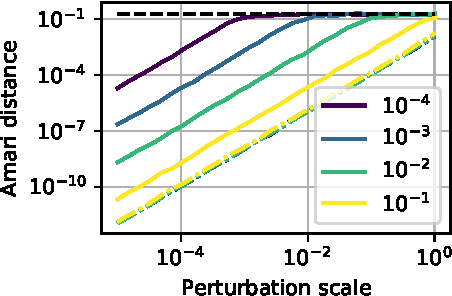
\includegraphics[width=\textwidth]{figures/multicca_gap_jd.pdf}
  %   \end{center}
  % \end{column}
    % \end{columns}
    % \vspace{1em}

    \textbf{Solved by joint diagonalization}:
    \begin{itemize}
    \item Large gap between the first $k$ eigenvalues and other: the span of the
      $p$ leading eigenvectors is preserved: 
      $W_i \approx Q \tilde{W}_i$.
    \item Recover $Q$ by joint diagonalization of $Q \tilde{W}_i \frac1{n}X_i X_i^{\top} \tilde{W}_i^{\top}Q^{\top}$
    \end{itemize}

    \vspace{0.5em}
    \textbf{Last steps}: Find scalings and noise variances (see paper)
  \end{block}

  % \vspace{0.5em}
  Related work: SRM~\cite{chen2015reduced}, MVICA~\cite{richard2020modeling},
  CanICA~\cite{varoquaux2010group}, IVA~\cite{anderson2014independent}.
  
  \vspace{0.5em}
  \begin{block}{Separation performance depending on the density of sources}
    Data generated with the ShICA model ($m=4$ views, $k=5$ components). Non-Gaussian sources have Laplace densities.\\
    {
      \vspace{1em}
      % \begin{figure}
        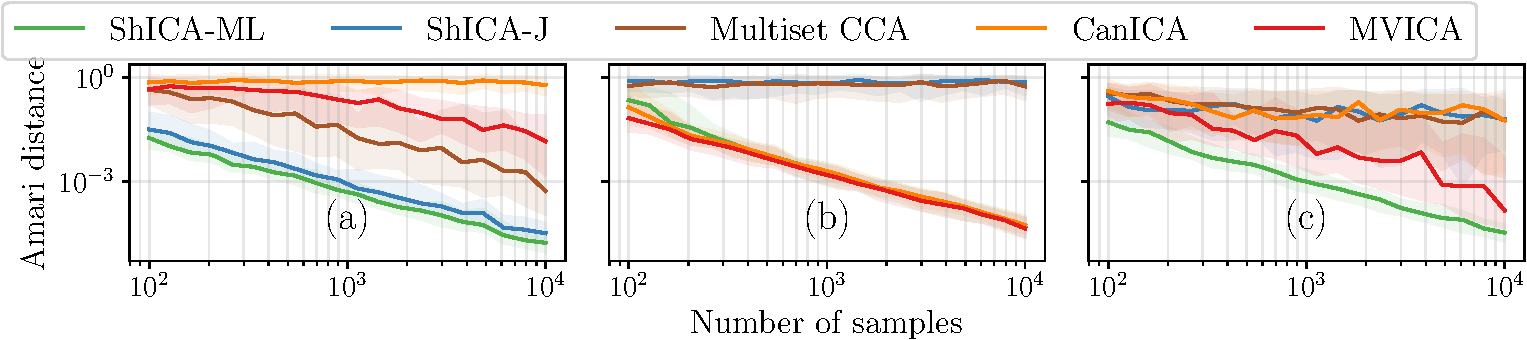
\includegraphics[width=\textwidth]{./figures/identifiability.pdf}\\
        % \caption{
          (a) Gaussian components with noise diversity
          (b) non-Gaussian components without noise diversity
          (c) Half of components are Gaussian with noise diversity, the other half is
          non-Gaussian without diversity
          % }
      % \end{figure}
    }
  \end{block}


\end{column} % End of the second column
\begin{column}{\sepwid}\end{column} % Empty spacer column

\begin{column}{\onecolwidthree} % The third column


    \begin{block}{Reconstruction experiment fMRI}
      \vspace{-0.5em}
      \begin{columns}
        \begin{column}{0.35 \textwidth}
          \begin{itemize}
          \item Subjects exposed to the same stimuli
          \item 80\% runs used to learn unmixing matrices
          \item In remaining runs we reconstruct the data of 20\% of the
            subjects using the other subjects.
          \end{itemize}
      \end{column}
      \begin{column}{0.65 \textwidth}
          \begin{center}
            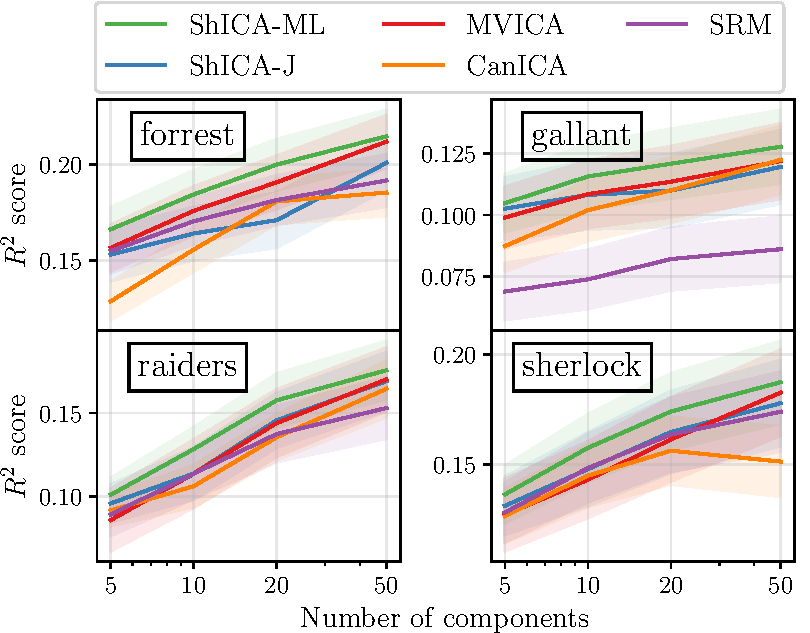
\includegraphics[width=\textwidth]{./figures/reconstruction.pdf}
          \end{center}
      \end{column}
      \end{columns}
    \end{block}

    \vspace{-1em}
    \begin{block}{MEG Phantom experiment}
      \begin{columns}

        \begin{column}{0.37 \textwidth}
          \begin{itemize}
            \item 8 dipoles in a plastic head at different locations separately
              emit signal $S_{true}$ during $n$ epochs
            \item $20$ sources are estimated: the best one is compared with $S_{true}$.
          \end{itemize}
    \end{column}

      \begin{column}{0.63 \textwidth}
    \begin{center}
      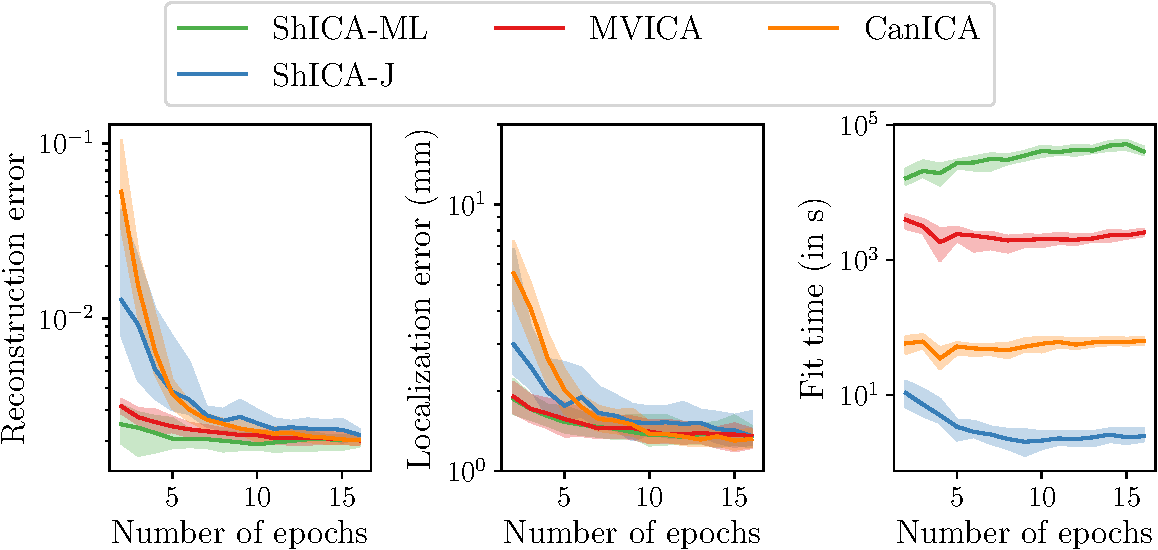
\includegraphics[width=1\textwidth]{./figures/meg_phantom_neurips.pdf}
    \end{center}
  \end{column}
    \end{columns}
  \end{block}

%----------------------------------------------------------------------------------------
%	CONCLUSION
%----------------------------------------------------------------------------------------


%----------------------------------------------------------------------------------------
%	REFERENCES
%----------------------------------------------------------------------------------------

\vspace{-1em}
\begin{block}{References}
  \nocite{*} % Insert publications even if they are not cited in the poster
    \printbibliography
\end{block}

\vspace{-1em}
  \small{
    \textbf{Acknowledgment} This work was supported by the European
    Union's Horizon 2020 Framework Programme (Grant Agreement No. 945539 Human Brain
    Project SGA3), the KARAIB AI chair (ANR-20-
    CHIA-0025-01), the SLAB ERC-StG-676943 and the BrAIN AI chair (ANR-20-CHIA-0016),
    the ANR "Investissements d'avenir" program (ANR19-P3IA-0001
    PRAIRIE 3IA Institute) and a CIFAR Fellowship.
  }

%----------------------------------------------------------------------------------------
%	ACKNOWLEDGEMENTS
%----------------------------------------------------------------------------------------

%----------------------------------------------------------------------------------------
%	CONTACT INFORMATION
%----------------------------------------------------------------------------------------
    

%----------------------------------------------------------------------------------------

\end{column} % End of the third column


\end{columns} % End of all the columns in the poster

\end{frame} % End of the enclosing frame

\end{document}
